\chapter{Methodology\label{cha:chapter3}}
This section determines the requirements necessary for X. This includes the functional aspects, namely Y and Z, and the non functional aspects such as A and B.

\section{Overview\label{sec:chapter3:overview}}

% In this chapter you will describe the requirements for your component. Try to group the requirements into subsections such as 'technical requirements', 'functional requirements', 'social requirements' or something like this. If your component consist of different partial components you can also group the requirements for the corresponding parts.

% Explain the source of the requirements.

% Example: The requirements for an X have been wide
% ly investigated by Organization Y.

In his paper about Z, Mister X outlines the following requirements for a Component X.

% \section{Technical Requirements\label{sec:techreq}}

% The following subsection outlines the technical requirements to Component X.

% \subsection{Sub-component A\label{sec:reqsuba}}

% \textbf{Interoperability}
% \\
% Lorem Ipsum...
% \\
% \\
% \textbf{Scalability}
% \\
% Lorem Ipsum...

% \subsection{Sub-component B\label{sec:reqsubb}}

% Lorem Ipsum...

% \section{Social Requirements\label{sec:socreq}}

% Component X must compete with Y. Hence, it is required to provide an excellent usability. This includes ...

\section{Hysteretic neural networks\label{sec:chapter3:hnn}}
\subsection{Play and Prandtl-Ishlinskii networkds\label{sec:chapter3:play-and-pi-networks}}
\\
Consider $K > 0$ play operators. Each of them maps an initial state $p_{0}^{k} \in \mathbb{R} $ and an input sequence $x_1, x_2, \ldots$ to an output sequence $p_{1}^{k}, p_{2}^{k}, \ldots \ $, i.e.,

% \begin{equation}\label{eqn:input_to_op_output_mapping}
\begin{equation*}
  p_{0}^{k}, (x_1, x_2, \ldots) \mapsto (p_{1}^{k}, p_{2}^{k}, \ldots), k = 1, \ldots, K
\end{equation*}

The $k$th play operator is given by:

\begin{equation}\label{\eqn:chapter3:play-operator}
  p_{n}^{k} = G(x_{n}, p_{n-1}^{k}, w^{k}) := p_{n-1}^{k} + \Phi(w^{k} x_{n} - p_{n-1}^{k}), n = 1, 2, \ldots
\end{equation}

where $w^{k}$ are parameters and

\begin{equation}\label{\eqn:chapter3:phi}
  \begin{aligned*}
    \Phi(x) =
    \begin{cases}
      x - \frac{1}{2}, & x > \frac{1}{2} \\
      0,               & -\frac{1}{2} <= x <= \frac{1}{2} \\
      x + \frac{1}{2}, & x < \frac{1}{2}
    \end{cases}
  \end{aligned*}
\end{equation}

See Fig. \ref{fig:chapter3:phi}

\begin{figure}[htb]
  \centering
  \resizebox{8cm}{!}{\documentclass{standalone}
\usepackage{tikz}
\begin{document}
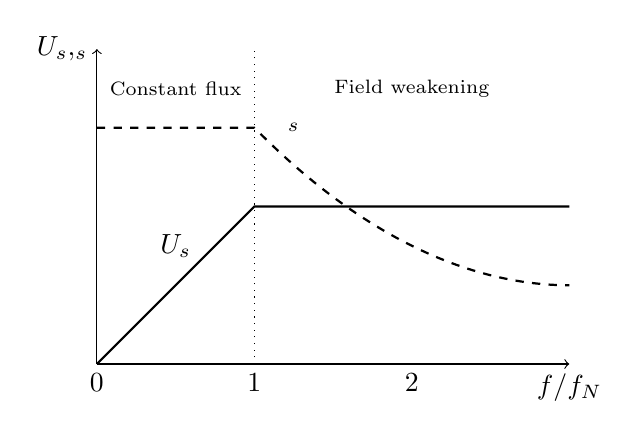
\begin{tikzpicture}
% horizontal axis
\draw[->] (0,0) -- (6,0) node[anchor=north] {$f/f_N$};
% labels
\draw	(0,0) node[anchor=north] {0}
		(2,0) node[anchor=north] {1}
		(4,0) node[anchor=north] {2};
% ranges
\draw	(1,3.5) node{{\scriptsize Constant flux}}
		(4,3.5) node{{\scriptsize Field weakening}};

% vertical axis
\draw[->] (0,0) -- (0,4) node[anchor=east] {$U_s,\varPsi_s$};
% nominal speed
\draw[dotted] (2,0) -- (2,4);

% Us
\draw[thick] (0,0) -- (2,2) -- (6,2);
\draw (1,1.5) node {$U_s$}; %label

% Psis
\draw[thick,dashed] (0,3) -- (2,3) parabola[bend at end] (6,1);
\draw (2.5,3) node {$\varPsi_s$}; %label

\end{tikzpicture}
\end{document}
}
  \caption{$\Phi(x)$}\label{fig:chapter3:phi}
\end{figure}

It can be represented as a recurrent neural network, see Fig. \ref{fig:chapter3:phi}. Note that in such a form the network is not feed-forward.
One can unfold it to make it feed-forwaard, see Fig. \ref{fig:chapater3:play-operator}

*Definition 1.1.* We call this network a \textsl{play network}. If there are \textsl{m} elements in the sequence ${x_n}$, we say the unfolded network is \textsl{m-unfolded}

For example, the network in Fig. \ref{fig:chapter3:unfolded-nn} is 2-unfolded.


\subsection{Play layers and Prandtl-Ishlinskii networkds\label{sec:chapter3:play-layers-and-pi-networks}}

\subsection{Training a PI network\label{sec:chapter3:training-pi-network}}
Assume we are given an input sequence $x_1, x_2, \ldots, x_N$ and an output sequence $q_1, q_2, \ldots, q_N$. We perform the following steps in cycle until convergence.

\begin{enumerate}
\item Preparing initial states for the $m$-unfolded network: Fix a vector of initial states $P_0$ and all the weights (denoted by $W$). For each $k=1, \ldots, K$, we calculate recursively $p_{1}^{k}, p_{2}^{k}, \ldots, p_{N}^{k}$ by formula \ref{eqn:chapter3:play-operator}. We denote the corresponding (intermediate) states of the \textbf{PI} operator by
  \begin{equation*}
    P_n = (p_{n}^{1}, \ldots, p_{n}^{K}), n = 1, \ldots, N.
  \end{equation*}
\item Preparing inputs for the $m$-unfolded network: We fix $m$ and group the input sequence into $m$-tuples:
  \begin{equation*}
    \mathbf{x_1} := (x_1, \ldots, x_m), \quad \mathbf{x_2} := (x_2, \ldots, x_{m+1}), \quad \ldots,
  \end{equation*}
  which gives $M := N-m$ tuples $\mathbf{x_1}, \ldots, \mathbf{x_M}$. Next we form a new set of inputs for the $m$-unfolded network, attaching the vectors of intermediate states:
  \begin{equation*}
    \mathbf{y_1} := (P_0, \mathbf{x_1}), \quad \mathbf{y_2} := (P_1, \mathbf{x_2}), \quad \ldots,
  \end{equation*}

\item Training the $m$-unfoled network: We train by stochstic gradient descent the feed-forward $m$-unfolded \textbf{PI} network
  \begin{equation*}
    \mathbb{R}^{K} \times \mathbb{R}^{m} \ni \mathbf{y} \mapsto F_{m}(\mathbf{y}) \in \mathbb{R}^m
  \end{equation*}
  with the inputs $\mathbf{y_1}, \ldots, \mathbf{y_M}$ and the true targets $mathbf{q_1}, \ldots, mathbf{q_M}$, where
  \begin{equation*}
    \begin{aligned*}
      \mathbf{q_1} = (q_1, \ldots, \q_m), \quad \mathbf{q_2} = (q_2, \ldots, q_{m+1}), \quad \ldots
    \end{aligned*}
  \end{equation*}

\item We update the initial state $P_0$:
  \begin{equation*}
    P_{0}^{new} := P_{0} - \nabla_{P_0} (F_m(P_0, \mathbf{x_1}) - \mathbf{q_1})^2
  \end{equation*}
\end{enumerate}

\subsection{General hysteretic networks\label{sec:chapter3:general-hysteretic-networks}}
A general network may consist of several play layers (and perhaps standard layers). We can such a network \textsl{hysteretic}, and denote
\begin{equation*}
  p_n = F(X_n, W)
\end{equation*}
where $X_n = (x_1, \ldots, x_n)$ and $w$ is a vector of all weights of the network.
